
%%%%%%%%%%%%%%%%%  B

\newpage

\begin{justify}

    {\bf Β} ΄Εστω
    \[ Y (t) = X \cos(2\pi F_0 t + \Phi),  \]
    όπου \( X \sim \mathcal{N} (0, 1) \), \( \Phi \sim U[0, 2\pi) \), και \( X \), \( \Phi \) ανεξάρτητες τυχαίες μεταβλητές.
    \end{justify}
    
    
    \begin{justify}
        (5) Να σχεδιάσετε σε κοινό \textlatin{plot} 5 υλοποιήσεις της.
    \end{justify}

%%%%%%PLOT
\begin{center}
    \centering
    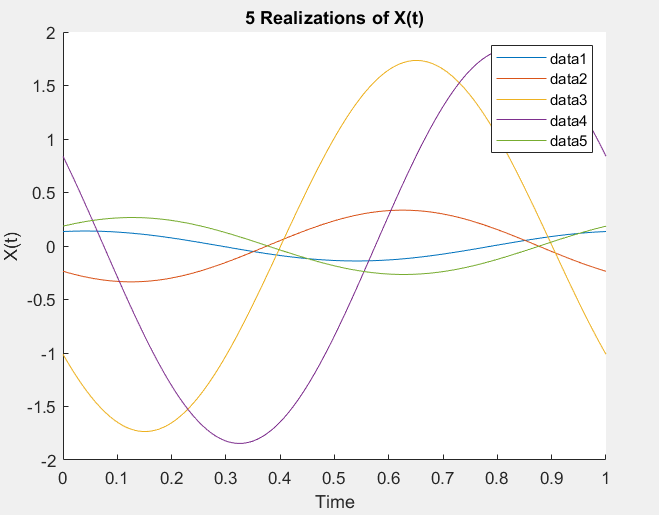
\includegraphics[width=0.8\textwidth]{BETA/Images/b.png} % Adjust width as neededfilename of your images
\end{center}


\begin{justify}
    και ο κώδικας \textlatin{Matlab}:
\end{justify}

\vspace{-1cm}

%%%%%%%%MATLAB code
\textlatin{
    \lstinputlisting[language=Matlab]{BETA/Matlab/b.m}
} 

    
    \begin{justify}
        (10) Να υπολογίσετε τις ποσότητες \( E[Y (t)] \) και 
        \( R\textsubscript{\textlatin{YY}} (t + \tau, t) = E[(Y (t + \tau )Y (t)]. \) 
        Τι διαπιστώνετε\textlatin{;}
    \end{justify}


    \begin{justify}
        {\bf Λύση:}\\\\
        \textlatin{i)}Αρχικά έχουμε:
        \[
        E[Y (t)] = E[X(t)\cdot \cos(2\pi F_0 t + \Theta)] = E[X(t)]\cdot
        E[\cos(2\pi F_0 t + \Theta] \tag{1}   
        \] 
         Επειδή οι \( X \) και \( \Theta \) είναι ανεξάρτητες 
         τυχαίες μεταβλητές, έχουμε:
         \[
            E[X(t)] = E[\sum_{n=0}^{N-1}X_n\phi(t-nT)] = 
            \sum_{n=0}^{N-1}E[X_n\phi(t-nT)] = \sum_{n=0}^{N-1}E[X_n]
            \phi(t-nT) = 0 \tag{2}
         \]
         διότι τα $X_n$ προκύπτουν από ομοιόμορφη κατανομή. 
         Επομένως από τις σχέσεις (1) και (2) προκύπτει:
         \[
            E[Y(t)] = 0 
         \]
    \end{justify}

    \begin{justify}
        \textlatin{ii)}Στη συνέχεια, έχουμε:
        \[
        R\textsubscript{\textlatin{YY}}(t+\tau, t) = E[Y(t+\tau)\cdot Y(t)] = E[X(t+\tau)
        \cdot\cos(2\pi f_0(t+\tau) + \Theta)\cdot X(t)
        \cdot\cos(2\pi f_0 t + \Theta)] \
        \]
        \[
           = E[X(t+\tau)\cdot X(t)]\cdot E[\cos(2\pi f_0(t+\tau) + \Theta) 
           \cdot \cos(2\pi f_0(t) + \Theta) ]
        \]
        θα θέσουμε $t+\tau=t_1$ και $t=t_2$, οπότε:
        \[
            E[X(t+\tau)\cdot X(t)] = E[X(t_1)\cdot X(t_2)] =
            Ε[\sum_{n=-\infty}^{\infty}X_n\phi(t_1-nT)\cdot
            \sum_{n=-\infty}^{\infty}X_n\phi(t_2-nT)]
        \]
        \[
            = E[\sum_{n=-\infty}^{\infty}X_n^2\cdot \phi(t_1-nT) \phi(t_2-nT)] 
            = \sum_{n=-\infty}^{\infty}E[X_n^2]\cdot \phi(t_1-nT)\phi(t_2-nT) =
            \]
\end{justify}

\newpage

\begin{justify}
    \[
        = \sum_{n=-\infty}^{\infty} \sigma_X^2 \cdot \phi(t+\tau-nT)\phi(t-nT)     
    \]
    και επιπλέον έχουμε:
    \[
        Ε[\cos(2\pi f_0 t_1 + \Theta) \cdot \cos(2\pi f_0 t_2 + \Theta)] =
        E[\frac{1}{2}\cos(2\pi f_0(t_1-t_2)) + 
        \frac{1}{2}\cos(2\pi f_0(t_1+t_2) + 2\Theta)]=
    \]
    \[
        E[\frac{1}{2}\cos(2\pi f_0(t_1-t_2))] +
        E[\frac{1}{2}\cos(2\pi f_0(t_1+t_2) + 2\Theta)]=   
        \frac{1}{2}\cos(2\pi f_0(t_1-t_2)) + 0 = 
    \]
    \[
        \frac{1}{2}\cos(2\pi f_0(t+\tau-t) = \frac{1}{2}\cos(2\pi f_0\tau)  
    \]
    Επομένως:
    \[
        E(Y(t+\tau)Y(t)) = \left ( \sum_{n=-\infty}^{\infty} \sigma_X^2 \cdot \phi(t+\tau-nT)\phi(t-nT)  \right )
        \cdot \frac{1}{2}\cos(2\pi f_0\tau).
    \]
\end{justify}

    
    \begin{justify}
        (5) Να υπολογίσετε τη φασματική πυκνότητα ισχύος, \( S_Y (F) \).
    \end{justify}

    \begin{justify}
        {\bf Λύση:}\\\\
        Η Φασματική πυκνότητα ισχύος της \( Y(t) \) 
        ορίζεται ως \( S_Y(F) = \mathcal{F}\{\overline{R}_Y\} \)
        με $\overline{R}_Y(\tau) \xrightarrow{\mathcal{F}} \overline{R}_Y(F).$
        Άρα έχουμε:
        \[
            \overline{R}_Y(\tau) = \frac{1}{T} 
            \int_{-\frac{T}{2}}^{\frac{T}{2}} R_{YY}(t + \tau, t) \, dt 
            = \frac{1}{T} \int_{-\frac{T}{2}}^{\frac{T}{2}} R_{XX}(t + \tau, t) 
            \cdot \frac{1}{2} \cos(2\pi f_0 \tau) \, dt  
        \]
        \[
          = \frac{1}{2T} \cos(2\pi f_0 \tau) \cdot 
          \int_{-\frac{T}{2}}^{\frac{T}{2}} R_{XX}(t + \tau, t) \, dt  
          = \frac{1}{2} \cos(2\pi f_0 \tau) \cdot \overline{R}_X(\tau)
        \]
        Άρα:
        \[
            S_Y(F) = \frac{1}{2} \mathcal{F} 
            \left\{ \cos(2\pi f_0 \tau) \cdot R_X(\tau) 
            \right\} = \frac{1}{4} \left( S_X(F + f_0) + 
            S_X(F - f_0) \right)
        \]
    \end{justify}